\documentclass{beamer}

\usepackage[utf8]{inputenc}
%\usepackage{beamerthemesplit}
\usepackage{url}
\usepackage{tikz}
\usepackage{alltt}
\usepackage{listings}
\usepackage{marvosym}
\usepackage{color}
\usepackage[multidot]{grffile}
\usepackage{multirow}
\usepackage{array}
\usepackage{setspace}
\usepackage{hyperref}
\usepackage{verbatim}
\usepackage{fancyvrb}
%\hypersetup{colorlinks=true, linkcolor=blue,  anchorcolor=blue,  
%citecolor=blue, filecolor=blue, menucolor=blue, pagecolor=blue,  
%urlcolor=blue} 
\lstset{keywordstyle=\bfseries\color{brown},
        stringstyle=\ttfamily,
        commentstyle=\color{blue}\textit,
        showstringspaces=false}

\useoutertheme{}
\usetheme{Madrid}
\graphicspath{{pics/}{global/}
{pics/I/}{pics/A1/}{pics/A2/}{pics/A3/}{pics/A4/}{pics/A5/}{pics/A6/}{pics/A7/}
}

\logo{
\includegraphics[height=1cm]{ProcessHorizontal}} 

\institute{Center for Computation and Technology\\Louisiana State University, Baton Rouge, LA}

\setbeamertemplate{navigation symbols}{} 

\title{CSC 7700: Scientific Computing}

% We want to use the infolines outer theme because it does not use a lot of
% space, but it also tries to print an institution and the slide
% numbers (which we might not want to show). Therefore, we here redefine the
% footline ourselfes - mostly a copy & paste from
% /usr/share/texmf/tex/latex/beamer/themes/outer/beamerouterthemeinfolines.sty
\defbeamertemplate*{footline}{infolines theme without institution and slide numbers}
{
  \leavevmode%
  \hbox{%
  \begin{beamercolorbox}[wd=.25\paperwidth,ht=2.25ex,dp=1ex,center]{author in head/foot}%
    \usebeamerfont{author in head/foot}\insertshortauthor
  \end{beamercolorbox}%
  \begin{beamercolorbox}[wd=.5\paperwidth,ht=2.25ex,dp=1ex,center]{title in head/foot}%
    \usebeamerfont{title in head/foot}\insertshorttitle
  \end{beamercolorbox}%
  \begin{beamercolorbox}[wd=.25\paperwidth,ht=2.25ex,dp=1ex,center]{date in head/foot}%
    \usebeamerfont{date in head/foot}\insertshortdate{}
  \end{beamercolorbox}}%
  \vskip0pt%
}

% Some useful commands
\newcommand{\abspic}[4]
 {\vspace{ #2\paperheight}\hspace{ #3\paperwidth}\includegraphics[height=#4\paperheight]{#1}\\
  \vspace{-#2\paperheight}\vspace{-#4\paperheight}\vspace{-0.0038\paperheight}}

\newcommand{\picw}[4]{{
 \usebackgroundtemplate{
 \color{black}\vrule width\paperwidth height\paperheight\hspace{-\paperwidth}\hspace{-0.01\paperwidth}
 \hspace{#4\paperwidth}\includegraphics[width=#3\paperwidth, height=\paperheight]{#1}}\logo{}
 \frame[plain]{\frametitle{#2}}
}}
\newcommand{\pic}[2]{\picw{#1}{#2}{}{0}}

\newcommand{\question}[1]{\frame{\frametitle{#1}
 \begin{centering}\Huge #1\\\end{centering}
}}


\usepackage{ragged2e}
\usepackage{amsmath}
\usepackage{listings}
\newcommand{\Heaviside}{\operatorname{\Theta}}

\subtitle[Module A]{{\large Module A: Basic Skills}\\*[0.3em]Lecture 5: 3D Visualization using Visit}
\author[\mbox{
\includegraphics[height=0.6em]{fl_300}\hspace{0.5em}Frank Löffler}]{Dr Frank Löffler}
\date{Fri, Sep 13 2013}
\usecolortheme[RGB={18,86,125}]{structure}


\begin{document}

\frame{\titlepage}

\begin{frame}
\frametitle{Installing Visit}
\begin{centering}
\href{https://wci.llnl.gov/codes/visit/executables.html}{https://wci.llnl.gov/codes/visit/executables.html}\\*[3em]
\begin{itemize}
 \item Linux
 \item Max OS X
 \item Windows
\end{itemize}
\end{centering}
\end{frame}

\begin{frame}
\frametitle{Data to visualize}
\begin{centering}
Download (checkout/update) dataset from class repository:\\
\href{https://svn.cct.lsu.edu/repos/courses/sci-comp-2013-public/coursework/A5/rho.rl4.h5}{https://svn.cct.lsu.edu/repos/courses/sci-comp-2013-public/coursework/A5/rho.rl4.h5}\\
\end{centering}
About the dataset:
\begin{itemize}
 \item 3D dataset
 \item time-series
 \item density of pulsating neutron star
\end{itemize}
About the Format:
\begin{itemize}
 \item HDF5
 \item Hierarchical Data Format
 \item data model, library, and file format for storing and managing data
 \item optimized for large datasets and parallel I/O
 \item portable
 \item free library (open source)
\end{itemize}
\end{frame}

\begin{frame}
\frametitle{Visualizing density oscillations}
\begin{itemize}
    \item Start Visit
    \item You can try enabling 3D acceleration, but at least on Intel graphics
	  chips this tends to make VisIt fail at startup.
    \item open the output file of your choice
\end{itemize}
\begin{center}
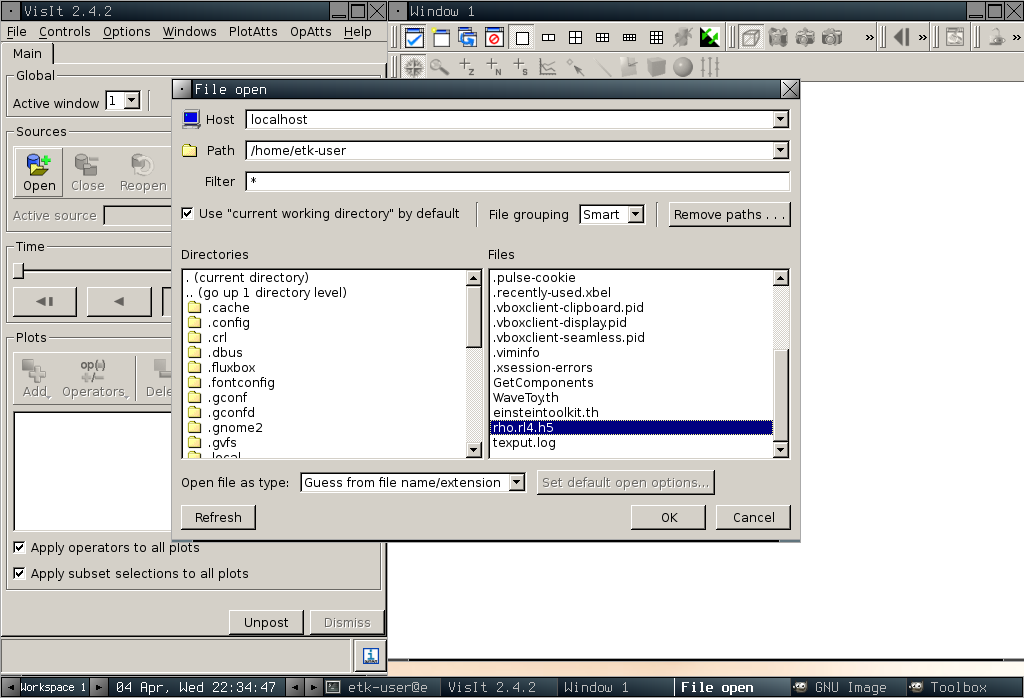
\includegraphics[height=48mm]{open_file}
\end{center}
\end{frame}

\begin{frame}
\frametitle{Visualizing density oscillations}
\begin{columns}
\column{60mm}
\begin{itemize}
\item add a pseudocolor plot from the "Plots" drop-down button
\item we will display a number of isocontour lines in the star to show its oscillations
\item we will use the \texttt{Isosurface} operator to compute the contour surfaces
\item \texttt{VisIt} also offers a \texttt{Contour} plot which however is limited in the transparency options compared to the \texttt{Isosurface}, \texttt{PseudoColor} combination we use
\end{itemize}
\column{60mm}
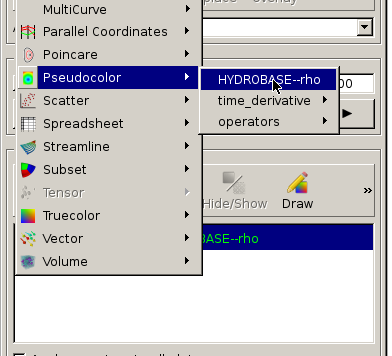
\includegraphics[width=60mm]{add_pseudocolor}
\end{columns}
\end{frame}

\begin{frame}
\frametitle{Visualizing density oscillations}
\begin{itemize}
\item add \texttt{Isosurface} operator from \texttt{Operators/Slicing/Isosurface}
\item add \texttt{Reflect} operator from \texttt{Operators/Transforms/Reflect}, to populate the ``missing'' octants
\end{itemize}
\begin{columns}
\column{60mm}
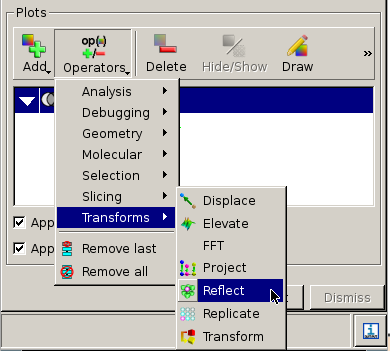
\includegraphics[width=60mm]{add_reflection}
\column{60mm}
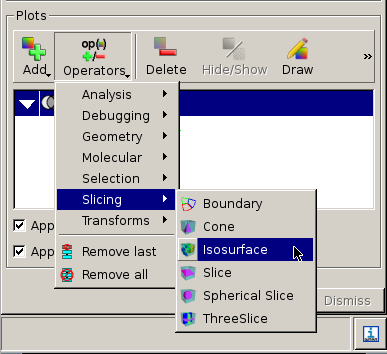
\includegraphics[width=60mm]{add_isosurface}
\end{columns}
\end{frame}

\begin{frame}
\frametitle{Visualizing density oscillations}
\begin{columns}
\column{60mm}
\begin{itemize}
\item double-click on the \texttt{Pseudocolor} entry in the list of plots to display its options page. Your might have to expand the list using the triangle shaped button on the left first
\item add transparency by reducing the opacity to about 25\% and set limits of $[10^{-8},10^{-3}]$ for the plot range. We will use the same range when creating isocontours in the next step
\item you have to click on \texttt{Apply} then on \texttt{Dismiss} to apply the new settings
\end{itemize}
\column{60mm}
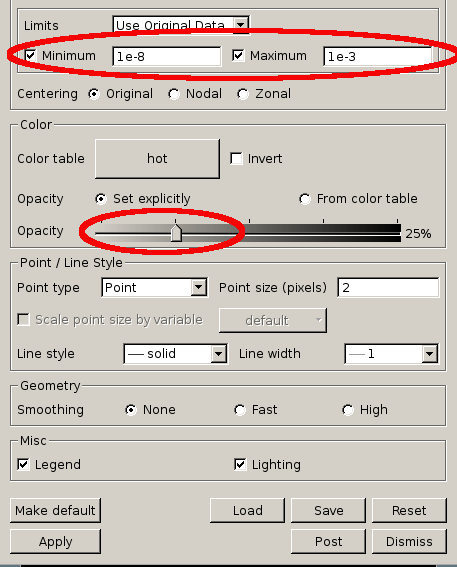
\includegraphics[width=60mm]{pseudocolour_options}
\end{columns}
\end{frame}

\begin{frame}
\frametitle{Visualizing density oscillations}
\begin{itemize}
\item double click on the \texttt{Reflect} operator, change to \texttt{3D} and activate all octants except the original ($+X+Y+Z$) one and the $+X-Y+Z$ one, change the reflection point to the origin.
\end{itemize}
\begin{center}
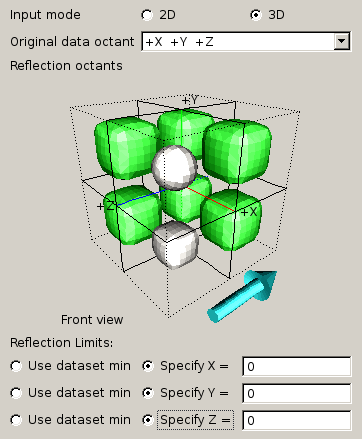
\includegraphics[height=60mm]{reflection_options}
\end{center}
\end{frame}

\begin{frame}
\frametitle{Visualizing density oscillations}
\begin{itemize}
\item double click on the \texttt{Isosurface} operator and select the range used for the \texttt{Pseudocolor} plot, use $6$ levels and leave the scaling at \texttt{linear}
\end{itemize}
\begin{center}
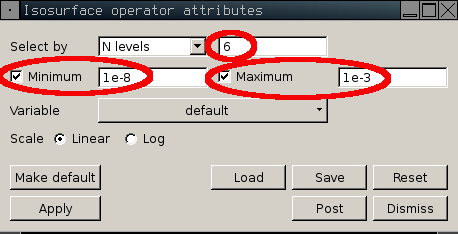
\includegraphics[width=60mm]{isocontour_options}
\end{center}
\end{frame}

\begin{frame}
\frametitle{Visualizing density oscillations}
\begin{itemize}
\item click on \texttt{Draw} to see how your plot looks like
\item rotate to an orientation that looks nice, by grabbing the plot with the mouse
\end{itemize}
\begin{center}
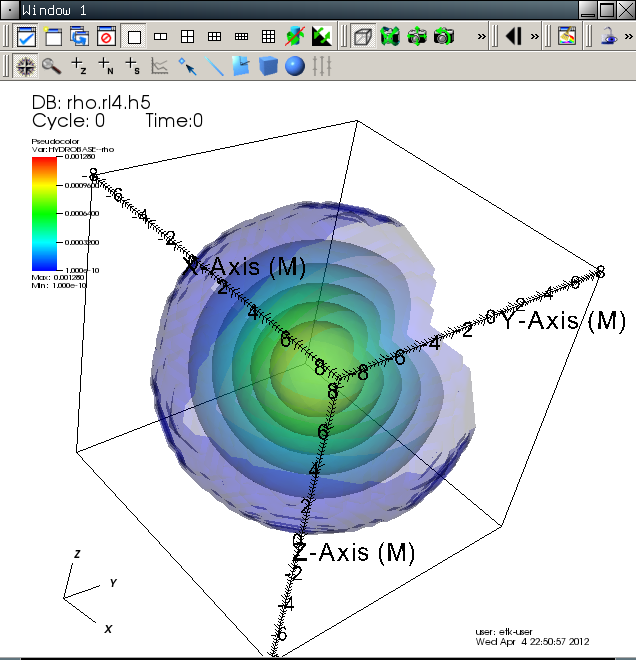
\includegraphics[width=60mm]{initial_plot_snapshot}
\end{center}
\end{frame}

\begin{frame}
\frametitle{Visualizing density oscillations}
\begin{columns}
\column{60mm}
\begin{itemize}
\item next we will change \texttt{VisIt}'s rendering options to add shadows and
change the background to something more attractive
\item unfortunately this means we will eventually loose the transparancy.
Though fiddling with the \texttt{Screen capture} option in \texttt{File/Save
Window Options...}. Experiment!
\item first though open the \texttt{Annotation} control page
\end{itemize}
\column{60mm}
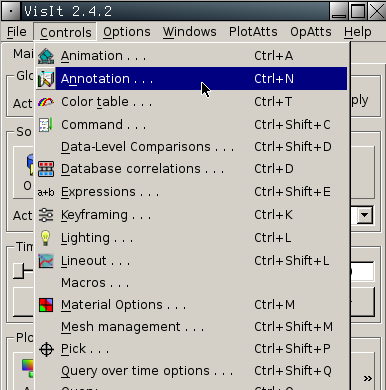
\includegraphics[width=60mm]{annotation_menu}
\end{columns}
\end{frame}

\begin{frame}
\frametitle{Visualizing density oscillations}
\begin{itemize}
\item in the \texttt{X-Axis} subtab of the \texttt{3D} tab, disable the axis title
\item repeat for the other two axes
\item in the \texttt{Colors} tab, change the background to black and the foreground to white
\item add a gradient to the background, with a dark gray as the second colour
\end{itemize}
\begin{center}
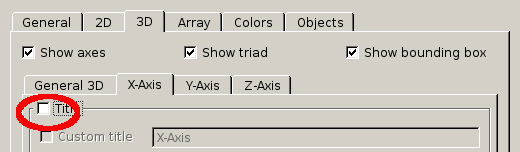
\includegraphics[width=58mm]{disable_x_axis}
\hfill
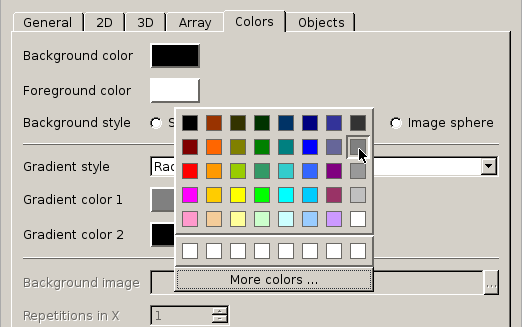
\includegraphics[width=58mm]{change_colour_scheme}
\end{center}
\end{frame}

\begin{frame}
\frametitle{Visualizing density oscillations}
\begin{columns}
\column{60mm}
\begin{itemize}
\item open \texttt{VisIt}'s rendering options from the \texttt{Options/Rendering...} menu
\item on the \texttt{Advanced} tab, enable \texttt{scalable rendering}, \texttt{Shadows} and \texttt{Depth Cueing}
\end{itemize}
\column{60mm}
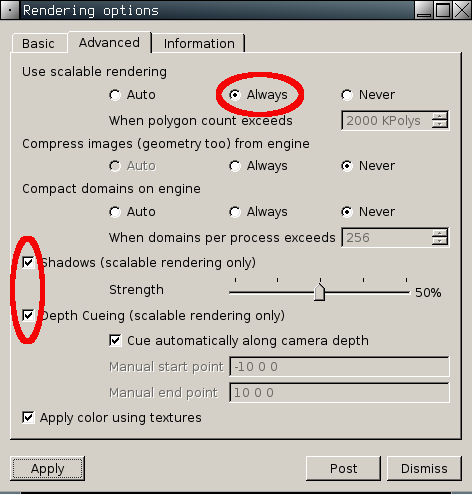
\includegraphics[width=60mm]{rendering_options}
\end{columns}
\end{frame}

\begin{frame}
\frametitle{Visualizing density oscillations}
\begin{itemize}
\item click on \texttt{Draw} to see how your plot looks like
\end{itemize}
\begin{center}
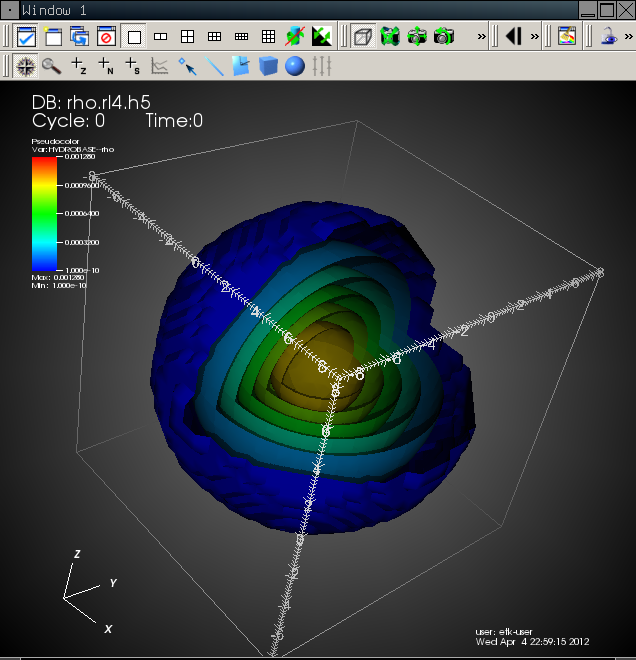
\includegraphics[width=60mm]{final_plot_snapshot}
\end{center}
\end{frame}

\begin{frame}
\frametitle{Visualizing density oscillations}
\begin{columns}
\column{60mm}
\begin{itemize}
\item in this last step we will let \texttt{VisIt} rendering frames of a small movie showing the oscillations
\item to start the movie wizard, select \texttt{Save movie...} from the \texttt{File} menu
\end{itemize}
\column{60mm}
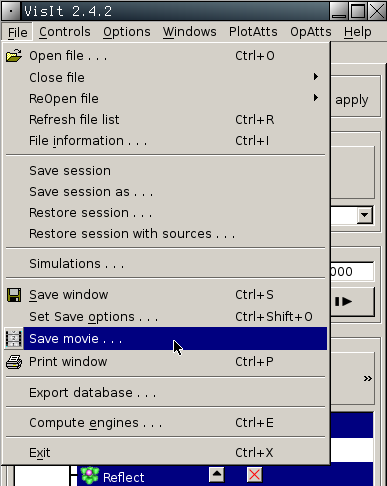
\includegraphics[width=60mm]{render_frames_menu}
\end{columns}
\end{frame}

\begin{frame}
\frametitle{Visualizing density oscillations}
\begin{columns}
\column{60mm}
\begin{itemize}
\item Finally, inside the wizard, change the frame size to approximately $640\times640$ pixels (multiples of $16$ are best)
\item choose \texttt{png} output
\item add the movie format to the list on the right using the \texttt{->} button
\item click on next and accept the defaults for all other steps, maybe choosing a different output directory for the frames
\end{itemize}
\column{60mm}
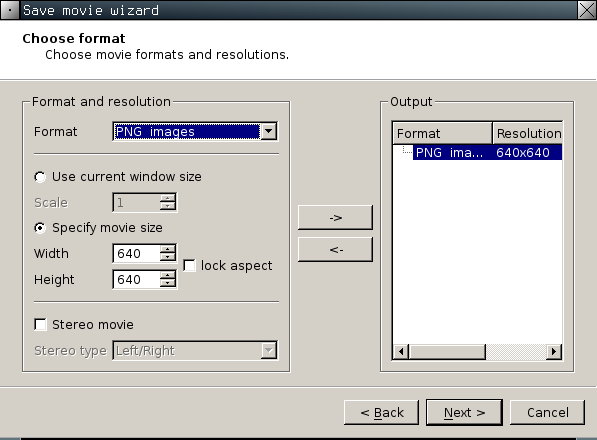
\includegraphics[width=60mm]{movie_frame_options}
\end{columns}
\end{frame}

\begin{frame}
\frametitle{Visualizing density oscillations}
\begin{itemize}
\item once \texttt{VisIt} is done, which will take some minutes, we can render the frames into an actual movie
\item for this, \texttt{cd} into the folder containing the frames and use, e.g., ffmpeg:
\begin{alltt}
ffmpeg -loop\_input -vframes 200 -qscale 1 -b 1000

-i movie\%04d.png movie.avi
\end{alltt}
\begin{itemize}
\item \texttt{-loop\_input} makes \texttt{ffmpeg} wrap around when looking for frames
\item \texttt{-vframes 200} is the number of frames to include in the movie, we set this to twice as many as we have actual frames, ie. the movie will loop twice
\item \texttt{-qscale 1} sets the quality scale for the encoder. $1$ is best quality.
\item \texttt{-b 1000} asks for a bitrate of $1000$ kilobits per second
\item \texttt{-i movie\%04d.png} tells \texttt{ffmpeg} the names of the input files, it accepts \texttt{printf} format specifiers to construct a file name based on the frame number. \texttt{ffmpeg} stops encoding once it generates a name for which no or no valid file is found.
\end{itemize}
\item play the movie, e.g., using \texttt{ffplay}
\end{itemize}
\end{frame}

\frame[containsverbatim]{\frametitle{Course Work}
Follow the previous steps to generate a sequence of images.
\begin{itemize}
 \item don't write-up these steps again in your report
 \item be sure to add all problems/obstacles you encountered
 \item select two images of the sequence - one close to (but not of) the first timestep,
       and one close (but not of) the end.
 \item Add these images to the report (include them in the pdf file, don't add the file separately)
 \item commit the single-file report to your repository (coursework/A5)
 \item Emphasis not on reproducing images identically, but on effort to gain experience
\end{itemize}
\vspace{2em}
\textbf{Due: Fri, Sep 20th 2013}
}

\end{document}
